\documentclass[10pt]{article}

\usepackage[a4paper,margin=0.2in]{geometry}
\usepackage{fontspec}
\usepackage{listings}
\usepackage{color}
\usepackage[framemethod=TikZ]{mdframed}
\usepackage[parfill]{parskip}
\usepackage{hyperref}
\usepackage{graphicx}

\setmainfont{Fira Sans}
\setmonofont{Fira Mono}
\newfontface\BoldMonoFont{Fira Mono Bold}[]

\pagenumbering{gobble}

\definecolor{gray}{RGB}{34, 34, 34}
\definecolor{red}{RGB}{248, 103, 78}
\definecolor{carminepink}{rgb}{0.92, 0.3, 0.26}
\definecolor{darkelectricblue}{rgb}{0.33, 0.41, 0.47}
\definecolor{antiquewhite}{rgb}{0.98, 0.92, 0.84}
\definecolor{columbiablue}{rgb}{0.61, 0.87, 1.0}
\definecolor{cadmiumgreen}{rgb}{0.0, 0.42, 0.24}
\definecolor{cobalt}{rgb}{0.0, 0.28, 0.67}
\definecolor{darkorange}{rgb}{1.0, 0.55, 0.0}
\definecolor{grannysmithapple}{rgb}{0.66, 0.89, 0.63}
\definecolor{atomictangerine}{rgb}{1.0, 0.6, 0.4}

\hypersetup{unicode=true,
            colorlinks=true,
            urlcolor=cobalt,
            breaklinks=true}

\lstset{
    inputencoding=utf8,
    extendedchars=true,
    aboveskip=0.5em,
    backgroundcolor=\color{white},
    basicstyle=\normalsize\ttfamily\color{black},
    breakatwhitespace=false,
    breaklines=true,
    captionpos=b,
    escapeinside={\%*}{*)},
    keywordstyle=\BoldMonoFont\color{carminepink},
    identifierstyle=\color{black},
    stringstyle=\color{cadmiumgreen},
    commentstyle=\color{darkelectricblue},
    showspaces=false,
    showstringspaces=false,
    showtabs=false,
    stepnumber=2,
}

\mdfsetup{
    nobreak=true,
    outerlinewidth=0,
    innerlinewidth=0,
    outerlinecolor=red!90,
    innerlinecolor=red!90,
    roundcorner=4pt,
    leftmargin=3,
    rightmargin=3,
    backgroundcolor=white,
    innertopmargin=0,
    innerbottommargin=10,
    innerleftmargin=9,
    innerrightmargin=9,
    splittopskip=\topskip,
}


\pagecolor{grannysmithapple}

\begin{document}

\twocolumn[
    \begin{@twocolumnfalse}
        \begin{mdframed}
            \begin{minipage}{24em}
                \vspace{1.0em}
                {
\includegraphics[scale=0.7]{tex/img/iohk-logo.png}}
            \end{minipage}
            \begin{minipage}{26.5em}
                \vspace{0.95em}
                \Large{LOGGING}
            \end{minipage}
            \begin{minipage}{2.5em}
                \vspace{1.0em}
                \href{https://github.com/input-output-hk/iohk-monitoring-framework}{GitHub}
            \end{minipage}
        \end{mdframed}
        \vspace{0.75em}
    \end{@twocolumnfalse}
]

\begin{mdframed}
    \section*{\href{https://github.com/input-output-hk/iohk-monitoring-framework/tree/master/contra-tracer}{contra-tracer}}

    A minimal implementation of \texttt{Tracer m a} is sufficient to start tracing observables in any code. Simply create a trace and add transformers to process the observables.

    \subsection*{Create a tracer}

    In this example, the terminal transformer outputs a text representation to the console:

    \begin{lstlisting}[language=Haskell]
let logTrace = showTracing stdoutTracer

showTracing
  :: (Show a)
  => Tracer m String
  -> Tracer m a

stdoutTracer
  :: (MonadIO m)
  => Tracer m String
    \end{lstlisting}

    \subsection*{Usage of the tracer argument in a function}

    For example:

    \begin{lstlisting}[language=Haskell]
handleBlockHeader logTrace = do
  ...
  curBlockHeader :: Header <- ...
  traceWith logTrace curBlockHeader
  ...
    \end{lstlisting}
\end{mdframed}

\begin{mdframed}
    \section*{\href{https://github.com/input-output-hk/iohk-monitoring-framework/blob/master/iohk-monitoring/src/Cardano/BM/Trace.lhs}{Hierarchy of traces}}

    The derived Trace m a type accepts LogObject for further processing and routing depending on the context name.

    A hierarchy of traces can be created by entering a local namespace with:

    \begin{lstlisting}[language=Haskell]
trace' <- appendName "deeper" trace
    \end{lstlisting}

    Observables on the new trace are annotated with the extended name.
\end{mdframed}

\begin{mdframed}
    \section*{\href{https://github.com/input-output-hk/iohk-monitoring-framework/blob/master/iohk-monitoring/src/Cardano/BM/Data/LogItem.lhs}{Privacy annotation}}

    The logged observables can be annotated with either\newline \texttt{Confidential} or \texttt{Public}. This will be taken into account when dispatching to the \texttt{katip} backend and its output scribes which are itself annotated to only process observables of a certain kind.
\end{mdframed}

\begin{mdframed}
    \section*{Trace with \href{https://github.com/input-output-hk/iohk-monitoring-framework/blob/master/iohk-monitoring/src/Cardano/BM/Data/Severity.lhs}{severity} annotation}

This code:

    \begin{lstlisting}[language=Haskell]
trace <- setupTrace (Left "config.yaml")
                    "test"
logInfo trace "Info"
logError trace "Error"
    \end{lstlisting}

leads to outputs:

    \begin{lstlisting}[language=Bash]
[iohk.test:Info:ThreadId 104] [2019-03-27 07:30:32.37 UTC] "Info"
[iohk.test:Error:ThreadId 104] [2019-03-27 07:30:32.37 UTC] "Error"
    \end{lstlisting}
\end{mdframed}

\begin{mdframed}
    \section*{\href{https://github.com/input-output-hk/iohk-monitoring-framework/blob/master/iohk-monitoring/src/Cardano/BM/Configuration/Model.lhs}{Configuration}}

The configuration is loaded on startup from a YAML file.

    \begin{lstlisting}[language=Haskell]
bTrace <- setupTrace (Left "config.yaml")
                     "base"
    \end{lstlisting}

    The returned trace in the namespace \texttt{"base"} will route all messages to the \texttt{Switchboard} which dispatches the messages to the backends according to configuration. The \texttt{katip} backend handles output to the console or log files, and also includes the log rotator.

The configuration contains mappings from the named context \texttt{LoggerName} to values changing the trace's behaviour.

Run:

    \begin{lstlisting}[language=Bash]
cabal new-run example-complex
    \end{lstlisting}

and access the editor on \href{http://localhost:13789}{http://localhost:13789}.
    
{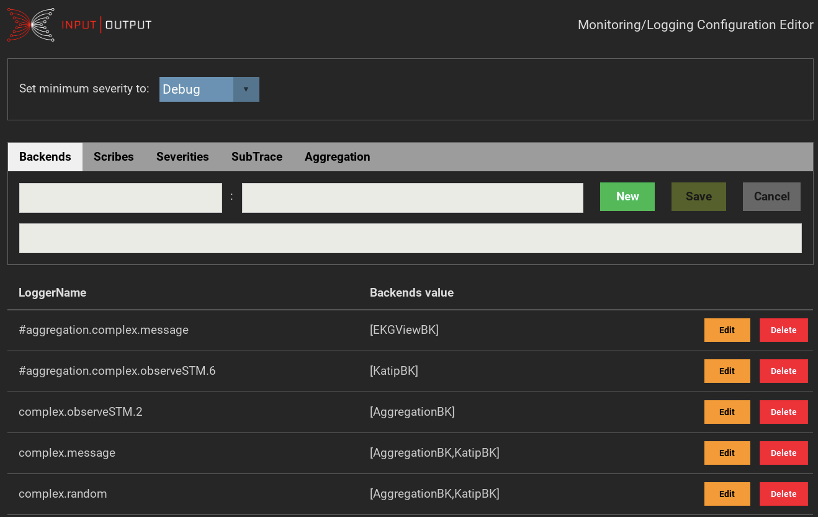
\includegraphics[scale=0.31]{tex/img/screen.png}}
    
Changes are effective immediately, because the changed configuration will be queried on arrival of every traced message.
\end{mdframed}

\end{document}
